\section{Metodología}
Se realizó un estudio aplicado, cuantitativo y experimental, con dos tomas de fotografías. Las imágenes se tomaron en una caja cerrada por tres lados, con una cámara web USB de 1280\,\texttimes\,720 píxeles y un anillo de 16 LED controlado por un ESP32-S3 (Figura 1). La luz se ajustó a un blanco neutro-cálido, porque una luz fría daba un tinte azulado. Una foto cada 3 segundos se guardó en JPEG (calidad 92) de hasta 800 píxeles de ancho, con tres formas de colocar los granos: en grupo, dispersos e individuales.

\begin{apafigure}{1}{Montaje de captura: interior de la caja y placa ESP32-S3}
\centering
\begin{minipage}[t]{0.48\linewidth}\centering
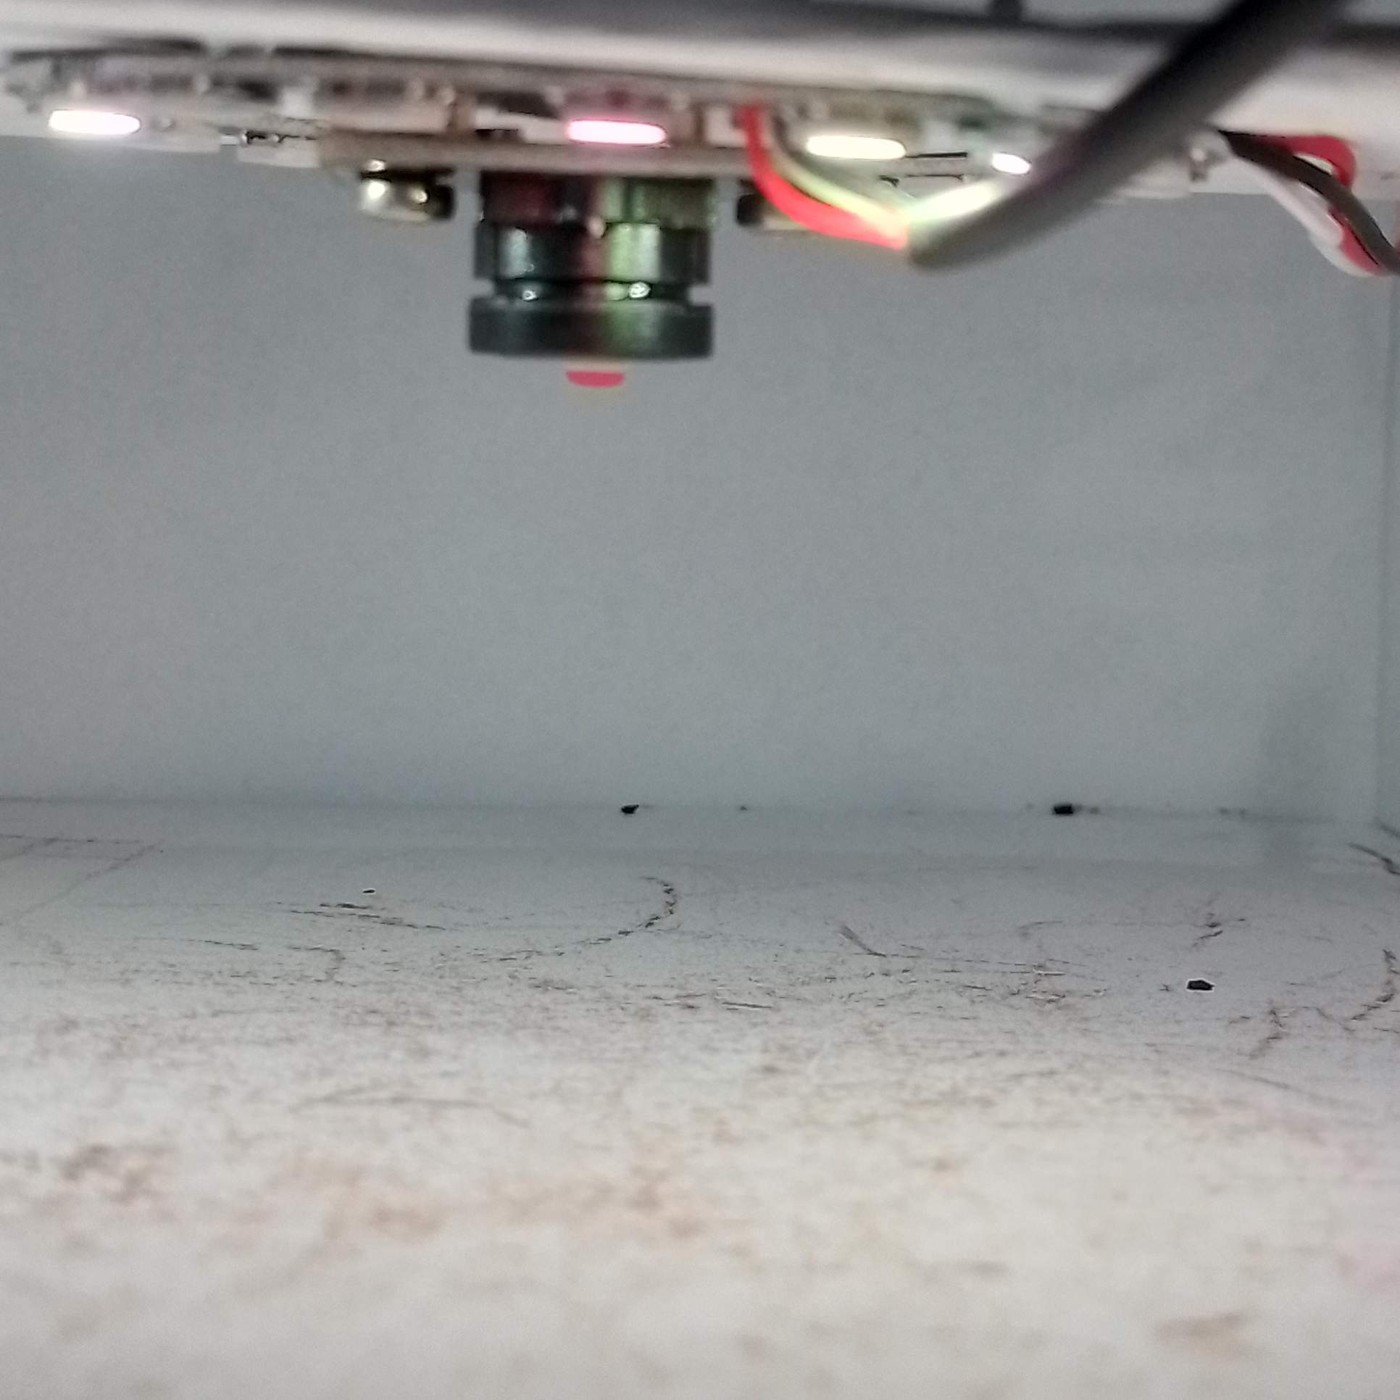
\includegraphics[width=\linewidth]{figures/fig_caja_interior.jpg}\\[2pt]{\small (a) Interior de la caja}
\end{minipage}\hfill
\begin{minipage}[t]{0.48\linewidth}\centering
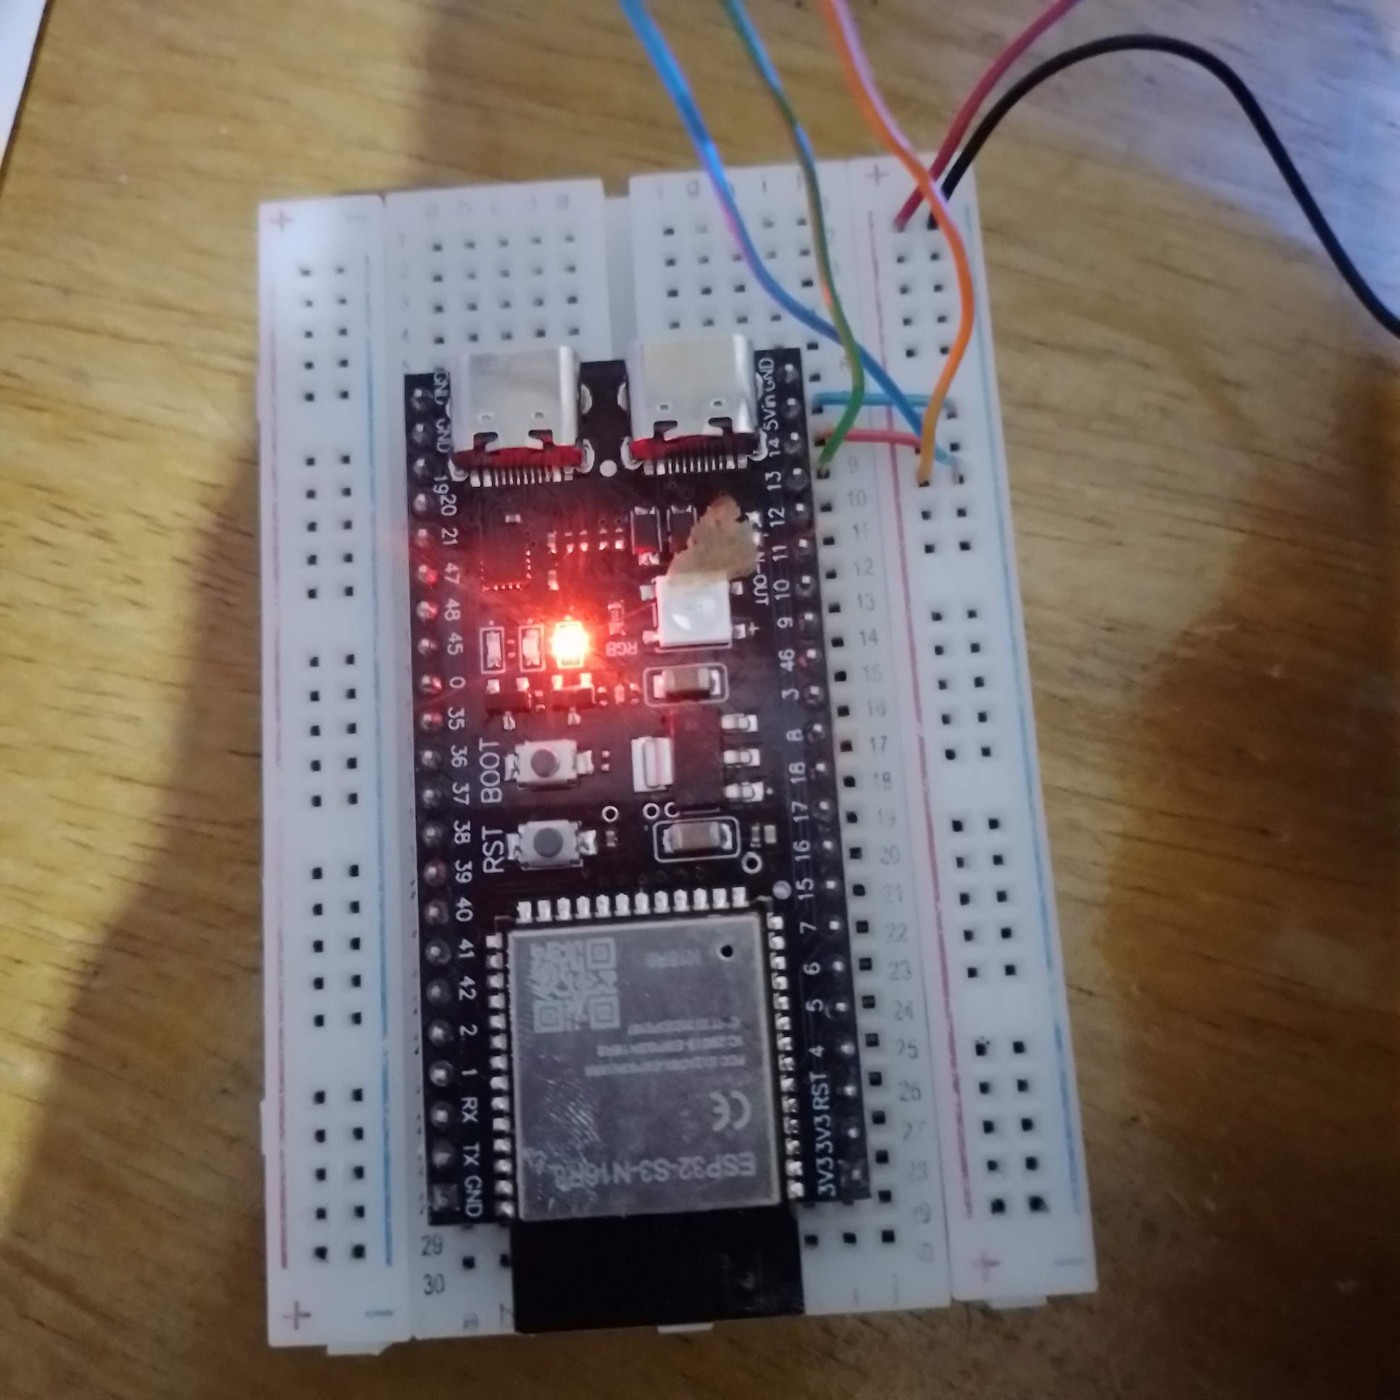
\includegraphics[width=\linewidth]{figures/fig_esp32s3.jpg}\\[2pt]{\small (b) Placa ESP32-S3}
\end{minipage}
\nota{Fotografías propias. (a) Cámara y LED en la parte superior de la caja. (b) Placa ESP32-S3 montada en una protoboard.}
\end{apafigure}

Se definieron siete clases: verde, claro, medio, medio oscuro, oscuro, quemado y fondo (papel vacío, manos y otros objetos). En la primera toma se grabaron 2.592 fotos sobre el papel inicial (verde 352, claro 370, medio 377, medio oscuro 372, oscuro 386, quemado 380 y fondo 355). Un filtrado automático con reglas propias descartó manos y guantes, fotos con pocas semillas visibles, desenfoque, mala exposición y mezcla de tuestes, y se recortó el centro de 450\,\texttimes\,450 píxeles para quitar el borde oscuro de la cámara, con lo que quedaron 2.328 fotos útiles.

En la segunda toma se volvieron a grabar todas las clases sobre una hoja blanca limpia, con la misma caja, cámara y luz, para que cada clase tuviera fotos con un mismo fondo; las fotos de la primera toma se conservaron, de modo que cada clase reúne fotos con los dos fondos. De 2.418 fotos tomadas, tras retirar capturas duplicadas en sucesión inmediata y aplicar el mismo filtrado y recorte, quedaron 830 útiles (verde 94, claro 78, medio 144, medio oscuro 123, oscuro 149, quemado 156 y fondo 86).

Las dos tomas se unieron en un conjunto de 3.158 fotos, que se dividió por bloques de cinco fotos consecutivas, ordenadas por fecha y hora de captura, para que fotos casi idénticas no quedaran a la vez en entrenamiento y prueba: 2.208 fotos de entrenamiento, 635 de validación y 315 de prueba. El orden de los bloques se mezcló con una semilla fija (42). Solo la carpeta de entrenamiento, con 2.207 fotos tras omitir un duplicado exacto, se subió a Teachable Machine; validación y prueba se guardaron para medir el modelo con fotos que nunca vio.

Se usó el modelo estándar de imágenes de Teachable Machine (224\,\texttimes\,224 píxeles en color, basado en una red tipo MobileNet) con los ajustes predeterminados de la herramienta, exportado en formato TensorFlow.js y convertido a ONNX para ejecutarlo con OpenCV sin instalar TensorFlow. Se verificó que la conversión conservó la salida del modelo original. La evaluación tuvo dos partes: la exactitud con las fotos de validación y prueba, separada según el fondo (papel inicial u hoja blanca, identificado por la fecha en el nombre de cada foto) y según la colocación de los granos (grupo, dispersos o individuales), y una prueba preliminar en vivo con la cámara del montaje, con el mismo recorte y tamaño que las fotos de entrenamiento.

Para medir el desempeño se calculó la exactitud, que es la proporción de fotografías que el modelo clasificó en la misma clase de la carpeta donde están guardadas (Ecuación 1), donde $A$ es el número de fotos acertadas y $N$ el número total de fotos evaluadas. Como la exactitud se mide con un número limitado de fotos, se calculó además su intervalo de confianza del 95 por ciento con el método de Wilson \citep{wilson1927} (Ecuación 2), donde $\hat{p}=A/N$ es la exactitud observada y $z=1{,}96$ es el valor de la distribución normal para ese nivel de confianza.

\begin{equation*}
\text{Exactitud}=\frac{A}{N}\tag*{[1]}
\end{equation*}

\begin{equation*}
\mathrm{IC}_{95}=\frac{\hat{p}+\dfrac{z^{2}}{2N}\;\pm\;z\sqrt{\dfrac{\hat{p}\,(1-\hat{p})}{N}+\dfrac{z^{2}}{4N^{2}}}}{1+\dfrac{z^{2}}{N}}\tag*{[2]}
\end{equation*}
